\documentclass{article}
\title{高校化学やり直し — モルと化学反応式}
\author{TeX 図書館}

\begin{document}

\section{読み方 — この本の地図と 3 つの道具}

高校化学でつまずくポイントは、ほぼ 1 か所に集約されています。\textbf{「物質量(モル)という目盛りに慣れていないうちに、反応式と濃度の計算へ進んでしまう」}こと。微粒子を数える道具としてモルを持ち出し、そのモルが化学反応式の係数とつながり、さらに溶液の中のモルとして濃度になる。この一本の線が見えていれば、問題は型に落とせます。

逆にこの線が切れていると単位がバラバラになり、「どの数字を割ればいいのか」が毎回思い出せなくなります。この本は、その一本の線をやり直す本です。前半で数え方を決め、中盤で反応の量関係へ進み、後半で実験の場面へ広げます。

\subsection{全 10 節の見取り図}

節の配分は次のとおりです。

\begin{enumerate}
\item 第 1〜2 節: 読み方と粒子モデル。物質を小さな粒の集まりとして見ます。
\item 第 3〜4 節: 原子量・分子量からモルへ。数え方の単位を決めます。
\item 第 5〜6 節: 化学反応式の係数合わせとモル計算。反応の量関係を扱います。
\item 第 7〜9 節: 溶液の濃度・酸と塩基・酸化還元。実験の場面へ広げます。
\item 第 10 節: まとめと次の一歩。
\end{enumerate}

各節の終わりには\textbf{解答の指針}を置きます。答えの丸写しではなく、どの式を立て、どの単位をつなぐかを書く欄です。まず自力で 5 分考えてから、その欄を開いてください。

\subsection{本書で使う式は 3 つだけ}

計算の道具は次の 3 つに絞ります。勝手な式は作りません。質量からモルへは、質量をモル質量で割ります。

\[ n = \frac{m}{M} \]

モルから個数へは、モル数にアボガドロ数を掛けます。逆に個数からモルへは割ります。

\[ N = n \times N_{\mathrm{A}} \]

そして溶液の中のモルは、体積で割って濃度に変えます。濃度とは「1 リットルの中にどれだけのモルがあるか」という言い換えにすぎません。

\(c = \frac{n}{V}\)

化学反応式の係数は、このモルの目盛りで読むと次のように書けます。水素 2 個分と酸素 1 個分が、水 2 個分に変わる、という意味です。

\[ 2\mathrm{H}_{2} + \mathrm{O}_{2} \rightarrow 2\mathrm{H}_{2}\mathrm{O} \]

\begin{quote}
\textbf{【注意】}\ 単位は式と一緒に書くこと。グラム、モル、リットルは別々の目盛りであり、換算せずに数字だけを並べても意味がありません。計算欄の最初に「何から何へ変えるか」を 1 行書いてから式を立てると、割り算の方向を間違えなくなります。
\end{quote}

\textbf{解答の指針:}\ まず問題文から求める量の単位を特定する(個数か、質量か、濃度か)。次に、その単位へ到達するまでの段取りを「質量 モル 個数」「濃度 モル 体積」のように言葉で並べる。並べたら、各段で使う式を 1 つずつ割り当て、最後に数字と単位を代入する。単位が式の上で約れて求める単位だけが残れば、計算は正しく進んでいます。

\section{物質と粒子モデル — 3 状態は間隔と運動の違い}

物質はどこまで割っても同じ性質の粒にたどり着きます。この粒を\textbf{粒子}と呼び、粒子モデルは「物質を粒子の集まりとして考える」見方です。化学変化を語るとき、どの議論もこの粒の数と並び方から始まります。したがって、ここが土台です。

見えている連続した塊が、実は離れた粒の集まりだという想像が難しいかもしれませんが、状態の違いを説明できるのはこのモデルだけです。同じ物質なのに固体・液体・気体で振る舞いが違うのは、粒が変わったからではなく、\textbf{間隔と動きやすさ}が変わったからです。

\subsection{3 状態のちがいは間隔と運動}

固体・液体・気体の違いを、粒子の位置と運動の言葉で整理します。

\begin{itemize}
\item \textbf{固体}: 粒子は密に規則正しく並び、その場で小刻みに振動します。形と体積がともに一定です。
\item \textbf{液体}: 粒子の間隔は固体とほぼ同じですが、並び方は不規則で、粒子は互いに滑り合います。形は変わり、体積は一定です。
\item \textbf{気体}: 粒子の間隔は大きく、互いに遠くを飛び回ります。形も体積も、入れた容器に従います。
\end{itemize}

状態変化で粒子そのものが消えたり新しくできたりすることはありません。変わるのは並び方と運動だけです。下の図は、この 3 状態を粒子の並びで並べたものです。

\begin{figure}
\centering
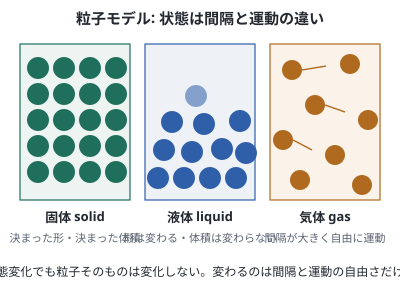
\includegraphics[width=0.8\textwidth]{figures/particle-model.svg}
\caption{粒子のモデル}
\end{figure}

\subsection{状態変化と化学変化を区別する}

同じ式を見ても、どちらが状態変化でどちらが化学変化かを区別できる必要があります。水の融解は、粒子の並び方が変わるだけの物理変化です。ここで水分子そのものは何も変わっていません。

\( \mathrm{H}_{2}\mathrm{O}(s) \rightarrow \mathrm{H}_{2}\mathrm{O}(l) \)

一方、水の電気分解では、水分子が壊れて水素分子と酸素分子に変わります。左辺と右辺で粒子の種類が違うのが化学変化のしるしです。

\[ 2\mathrm{H}_{2}\mathrm{O} \rightarrow 2\mathrm{H}_{2} + \mathrm{O}_{2} \]

同じ水でも、1 グラムと 1 リットルでは数が違います。密度はこの換算の入口であり、質量と体積をつなぐ量です。

\( \rho = \frac{m}{V} \)

\begin{quote}
\textbf{【定義】}\ 粒子モデルとは、物質を極小の粒子の集まりとみなし、状態や化学変化を「粒子の種類・数・間隔・運動」で説明する考え方をいう。状態変化は間隔と運動の変化、化学変化は粒子の種類と数の変化として区別される。
\end{quote}

\textbf{解答の指針:}\ 与えられた変化を「粒子の種類が変わったか、変わらないか」で判定する。種類が同じなら状態変化、種類が増え減りしたなら化学変化と分類する。そのうえで、前者は並び方と間隔、後者は粒子の数と係数の話に切り替える。図を思い出して、固体・液体・気体の並びを自分の言葉で 1 行ずつ説明できるようにしておけば十分です。

\section{原子量・分子量 — 数えるための目盛り}

粒子を数えるには、1 個あたりの質量を基準にする必要があります。しかし原子の質量はグラム単位では桁が小さすぎて扱いにくいため、化学では\textbf{相対}の目盛りを使います。これが原子量であり、分子量はその足し算です。

基準は炭素12原子で、その質量を 12.000 と定め、他の原子の質量をこの 12.000 に対する比で表します。水素は約 1.0、酸素は約 16.0 です。単位は付けません(相対の比であるため)。原子量が分かれば、分子量は構成原子の足し算だけで求まります。

\subsection{相対原子質量の考え方}

原子量は「炭素12 を 12.000 としたときの相対の値」です。したがって、同じ原子を何度測っても変わらず、原子そのものの絶対質量を表すわけでもありません。基準を変えれば数値全体も変わる、いわば目盛りの話です。

日常の身長と似ています。基準となる長さを決めておけば、他のものはすべてその比で表せるからです。化学式の中で原子記号の右下に書かれる数字の並びは、この目盛りを足し合わせた結果にほかなりません。

\subsection{分子量の求め方}

分子量は、分子を構成する各原子の原子量を、原子の数だけ掛けて足した値です。水を例にとると、水素原子が 2 個、酸素原子が 1 個なので、次のように計算します。

\[ M(\mathrm{H}_{2}\mathrm{O}) = 2 \times 1.0 + 16.0 = 18.0 \]

二酸化炭素は炭素 1 個と酸素 2 個からなります。

\[ M(\mathrm{CO}_{2}) = 12.0 + 2 \times 16.0 = 44.0 \]

塩化ナトリウムはイオン結晶ですが、化学式単位の見かけの質量も同じやり方で求めます。

\( M(\mathrm{NaCl}) = 23.0 + 35.5 = 58.5 \)

グルコースは原子の数が多いため、掛ける回数を間違えやすい典型例です。炭素 6、水素 12、酸素 6 と数え順に並べます。

\[ M(\mathrm{C}_{6}\mathrm{H}_{12}\mathrm{O}_{6}) = 6 \times 12.0 + 12 \times 1.0 + 6 \times 16.0 = 180.0 \]

\begin{quote}
\textbf{【例】}\ 「酸素 2 個分の質量を足す」と書くと 16.0 × 2 になり、48.0 となります。原子 1 個の原子量は 16.0 であって、分子の中の酸素は 2 個ある、と数え間違いの出る箇所を毎回確かめてください。
\end{quote}

\textbf{解答の指針:}\ 化学式を構成原子に分解し、記号ごとの個数を先に書き出す。次に個数 × 原子量を項目ごとに計算し、最後に足し合わせる。原子量の小数点以下の桁は問題の指示に従い、勝手に丸めない。分子量という語が出てきたら、単位を付けずに比の値であることを確認してから次へ進みます。

\section{モルとアボガドロ数 — 数える単位を決める}

原子量の目盛りが整えば、あとは「数え方」を決めればよいだけです。12 グラムの炭素には炭素原子が確かに多く、逆に水素 1 グラムにも同じだけの原子が含まれます。その\textbf{等しい個数}を 1 つの単位に束ねたものがモルです。

モルは打率や利率と同じく、単位にすぎません。ただし、グラムが質量の単位であるのに対し、モルは\textbf{個数の単位}である点に注意します。1 mol と書けば、どれの粒子であれ一定の個数を意味します。

\subsection{モルの定義}

1 mol に含まれる粒子の個数は、アボガドロ数と呼ばれ、次の値です。

\( N_{\mathrm{A}} = 6.02 \times 10^{23} \)

この数は基準の炭素12 が 12 グラム含まれるときに決まるため、原子量とつながります。つまり、原子量の数値と同数のグラムが 1 mol です。

\begin{quote}
\textbf{【定義】}\ モル(mol)とは、アボガドロ数 \( 6.02 \times 10^{23} \) 個の粒子の集まりを 1 単位とする物質量の単位をいう。摩爾質量 M(単位 g/mol)とは、1 mol の粒子の質量であり、数値は原子量・分子量と一致する。
\end{quote}

\subsection{質量とモルの相互換算}

質量からモルへの換算は、質量を摩爾質量で割るだけです。水 18.0 グラムは、分子量 18.0 で割るとちょうど 1 mol になります。

\[ n = \frac{m}{M} = \frac{18.0}{18.0} = 1.00 \]

逆に、モルから質量へは摩爾質量を掛けます。モルから粒子の個数へはアボガドロ数を掛けます。扱いやすい順に並べると次のとおりです。

\[ N = n \times N_{\mathrm{A}} \]

よく使う摩爾質量は、次の表のように暗記しておくと計算が速くなります。

\begin{center}
\begin{tabular}{|c|c|c|}
\hline
物質 & 化学式 & 摩爾質量 \\
\hline
水素分子 & H2 & 2.0 g/mol \\
水 & H2O & 18.0 g/mol \\
酸素分子 & O2 & 32.0 g/mol \\
塩化ナトリウム & NaCl & 58.5 g/mol \\
\hline
\end{tabular}
\end{center}

\textbf{解答の指針:}\ 問題文のグラムを見たら、まず摩爾質量で割ってモルに変える。個数が聞かれていれば、モルにアボガドロ数を掛ける。逆方向(個数からグラム)なら、先にモルへ戻してから摩爾質量を掛ける。換算は 1 ステップずつ行い、各段で必ず単位を書き添えること。「g と g/mol を割れば mol になる」と単位の演算で確認できるなら、式の向きは正しいはずです。

\section{化学反応式の係数合わせ — 守るべき 3 つの数}

化学反応式は、反応物と生成物を矢印で結んだ式です。書けるようになるだけで演習量は増えますが、本質は\textbf{係数}にあります。係数は勝手に付けるのではなく、守るべき数を揃えることで決まります。

守る対象は、各元素の原子の数です。左辺と右辺で同じ元素の個数が一致しなければ、質量保存則に反します。気体の反応や水溶液の反応では、電荷の合計を揃えることも加わります。まずは原子の数から始めます。

\subsection{反応式は何を約束しているか}

最も基本な水素と酸素の反応を書き下すと、左辺の水素原子は 4 個、右辺も 4 個、左辺の酸素原子は 2 個、右辺も 2 個になり、両辺が一致します。

\[ 2\mathrm{H}_{2} + \mathrm{O}_{2} \rightarrow 2\mathrm{H}_{2}\mathrm{O} \]

この式は同時に「水素 2 mol と酸素 1 mol が反応して水 2 mol ができる」という量関係を約束しています。係数は個数の比であり、モルの比でもあります。ここが第 6 節のモル計算へ通じる接点です。

\begin{quote}
\textbf{【注意】}\ 係数を変えると量関係が変わるため、安易に両辺全体を 2 倍してはいけません。係数は互いに素な整数の並びとして揃え、単純な約分が残らないようにします。状態記号や熱の記号は係数決めの妨げになるので、まず原子の数だけを見てください。
\end{quote}

\subsection{係数合わせの手順}

手順は固定です。次の 4 段階で進めます。

\begin{enumerate}
\item 両辺に現れる元素を 1 つ選び、片方にだけ出る元素があれば先にそこを 1 とおく。
\item 各元素の原子の個数を数え、不足している側の係数を原子の個数比で仮置きする。
\item 他の元素に係数を波及させ、端数が残ったら全体を整数倍する。
\item 全元素の個数を再点検し、最大公約数で約分して互いに素な係数にする。
\end{enumerate}

メタンの燃焼は、酸素が 2 つ目の元素として登場する典型例です。炭素 1 個に対し酸素 2 個が必要になり、生成物側へ配ると次の形になります。

\( \mathrm{CH}_{4} + 2\mathrm{O}_{2} \rightarrow \mathrm{CO}_{2} + 2\mathrm{H}_{2}\mathrm{O} \)

鉄の酸化は、2 元素の化合物が右辺に出てくる例です。鉄原子を 4 つにすると、右辺の鉄原子と整合し、酸素も揃います。

\[ 4\mathrm{Fe} + 3\mathrm{O}_{2} \rightarrow 2\mathrm{Fe}_{2}\mathrm{O}_{3} \]

カルシウム炭酸の熱分解は、3 つの物質が並ぶ型で、左辺を 1 とおけば右辺も自然に決まります。

\( \mathrm{CaCO}_{3} \rightarrow \mathrm{CaO} + \mathrm{CO}_{2} \)

\textbf{解答の指針:}\ 右辺か左辺のどちらかにだけ出る元素を探し、そこに最初の 1 を置く。そこから原子の個数比で隣接する係数へ伝播させ、小数が残ったら全体を整数倍して約分する。最後に元素ごとに左辺・右辺の個数を表にして数え、すべて一致したことを確認して完了とします。電荷が絡むイオン反応では、個数の代わりに両辺の電荷の合計を同じにする、と手順の 1 行目だけ差し替えます。

\section{モル計算ドリル — 反応式を量関係として読む}

係数が揃った反応式は、そのまま計算の表に読み替えられます。「2 H2 と 1 O2」は「水素 2 mol と酸素 1 mol」という意味だからです。ここからは、この読み替えを使って質量から質量へ進む練習をします。

ドリルの型は 1 つしかありません。まず片方の物質量をモルへ戻し、係数の比で相手のモルへ変換し、最後に必要な単位へ戻す。この 3 段変換を体に入れることが、この節の目的です。

\subsection{係数はモル比である}

アンモニアの合成を例に、係数の意味を量の言葉で確認します。1 mol の窒素と 3 mol の水素が反応すると 2 mol のアンモニアができます。

\( \mathrm{N}_{2} + 3\mathrm{H}_{2} \rightarrow 2\mathrm{NH}_{3} \)

したがって窒素と水素のモル比は 1 対 3 です。質量比にすると 28 対 6 で、モル比とは一致しません。係数から読めるのは\textbf{モル比}であり、質量比を係数から直接読むのは典型ミスです。

\begin{quote}
\textbf{【例】}\ 「水素 4.0 グラムを燃やしたとき、必要な酸素は何グラムか」を解くとします。4.0 グラムを 2.0 g/mol で割って 2.0 mol。係数比 2 対 1 で酸素は 1.0 mol。32.0 g/mol を掛けて 32.0 グラム。この並びが基本の 3 段です。
\end{quote}

\subsection{質量から質量への 3 段変換}

上で挙げた例を、手順として固定します。

\begin{enumerate}
\item \textbf{モルへ}: 与えられた質量を摩爾質量で割る。
\item \textbf{モル比}: 反応式の係数の比を使って、目的の物質のモルを求める。
\item \textbf{戻す}: 目的の物質の摩爾質量を掛けて、求められる単位へ戻す。
\end{enumerate}

第 1 段は質量 4.0 グラムを水素の摩爾質量 2.0 g/mol で割ります。

\( n = \frac{4.0}{2.0} = 2.0 \)

第 2 段は係数の比です。水素が 2 の位置に来る反応式では、酸素は 1 なので、酸素のモルは水素の半分になります。

\( n(\mathrm{O}_{2}) = \frac{1}{2} n(\mathrm{H}_{2}) = 1.0 \)

第 3 段は摩爾質量との掛け算です。酸素分子の摩爾質量は 32.0 g/mol なので、次のように求まります。

\[ m = 1.0 \times 32.0 = 32.0 \]

\textbf{解答の指針:}\ 「質量 モル モル 質量」の 3 段を先に書いてから数字を入れる。第 2 段では必ず反応式に戻り、係数の比を書き下す(この段を飛ばすと、質量比で答えてしまう典型ミスが出ます)。最後に単位を追って、求める物質の単位だけが残っているかを確認する。答えの数値の桁は、与えられたデータの有効数字に合わせます。

\section{溶液の濃度 — 1 リットルにどれだけ入れたか}

実験では物質をまわりの液体に溶かして使います。このとき「どれだけ入れたか」を質量と体積の 2 通りで表すため、濃度には大きく 2 種類があります。使い分ければよいだけですが、混同すると計算が壊れるので、定義から揃えます。

濃度とは、言い換えれば\textbf{溶液を分母に取った割合}です。分母を質量に取れば質量パーセント、体積に取れば体積モル濃度になります。どちらも「入れた物質の量を、溶液全体で割る」という同じ構造を持ちます。

\subsection{質量パーセント濃度}

質量パーセント濃度は、溶質の質量を溶液全体の質量で割り、100 を掛けた値です。海水の塩分などがこれに当たります。

\( w = \frac{m_{\text{溶質}}}{m_{\text{溶液}}} \times 100 \)

分母は溶媒ではなく\textbf{溶液}である点が要点です。食塩 5 グラムを水 95 グラムに溶かせば溶液は 100 グラムになり、濃度は 5 パーセントです。水 100 グラムに溶かしたと数えると、分母が 105 グラムになって答えがずれます。

\begin{quote}
\textbf{【定義】}\ 体積モル濃度 c(単位 mol/L)とは、溶液 1 リットルに含まれる溶質の物質量 n で定義される濃度をいう。すなわち c = n / V であり、V は溶質ではなく溶液全体の体積を指す。
\end{quote}

\subsection{体積モル濃度とその計算}

水溶液で最も広く使われる単位が mol/L です。定義式は 1 つだけです。

\[ c = \frac{n}{V} \]

この式は 3 通りに読み替えられます。濃度が欲しければモルを体積で割り、モルが欲しければ濃度と体積を掛け、体積が欲しければモルを濃度で割る。どれも同じ式の変形にすぎません。

\( n = c \times V \)

具体例として、0.50 mol/L の塩化ナトリウム水溶液 0.25 L に含まれる塩化ナトリウムのモルは、濃度と体積の積で求まります。

\[ c = \frac{n}{V} \quad \text{より} \quad n = 0.50 \times 0.25 = 0.125 \]

実験では、この原液を溶媒で薄めて使います。薄める前後で溶質のモルは変わらないという保存則が、希釈計算の根拠です。したがって、薄める前の濃度と体積の積は、薄め後のそれと等しくなります。

\textbf{解答の指針:}\ 求める量が濃度・モル・体積のどれかを先に特定し、c や n や V の 3 つの中に既知が 2 つあるかを数える。既知が 2 つあれば定義式の変形で解けます。モルへ戻る場面では、溶質の質量を摩爾質量で割ることを忘れずに添える。溶液体積が mL で与えられているときは、mol/L の定義に合わせて先に L へ換算してから計算します。

\section{酸と塩基の基礎 — 何を受け渡すか}

水溶液の性質を分けてきた酸と塩基は、本質的に\textbf{プロトン(水素イオン)の受け渡し}で結びついています。定義は立場によって 2 つありますが、高校で扱う反応はどちらの定義でも同じ姿にたどり着くため、両方を押さえておきます。

酸は水素イオンを出し、塩基は水素イオンを受け取ります。この授受が起きると、両者はほぼ必ず水と塩に変わります。この形を\textbf{中和}と呼び、滴定などの定量分析の土台になります。

\subsection{酸と塩基の定義}

アレニウスの定義では、水に溶かしたときに水素イオンを出すものが酸、水酸化物イオンを出すものが塩基です。塩酸は水の中で完全に電離し、次のような形になります。

\[ \mathrm{HCl} \rightarrow \mathrm{H}^{+} + \mathrm{Cl}^{-} \]

ブロンステッドの定義はさらに広く、水素イオンを受け取るものが塩基です。アンモニアは水と反応して水から水素イオンを奪うため、塩基として振る舞います。

\( \mathrm{NH}_{3} + \mathrm{H}^{+} \rightarrow \mathrm{NH}_{4}^{+} \)

\begin{quote}
\textbf{【定義】}\ 酸とは水素イオンを供与する物質、塩基とは水素イオンを受け取る物質をいう(ブロンステッド・ローリーの定義)。酸と塩基が反応して水と塩が生じる反応を中和という。
\end{quote}

\subsection{中和反応と塩}

中和の最小形は、水素イオンと水酸化物イオンが水になる反応です。ここに両辺の電荷が等しくなっている点にも注目してください。

\( \mathrm{H}^{+} + \mathrm{OH}^{-} \rightarrow \mathrm{H}_{2}\mathrm{O} \)

この 1 行を元素と対応させると、酸全体と塩基全体の反応として次のように書けます。左辺の塩酸と水酸化ナトリウムは、電離して出てきたイオン同士が引き合うのです。

\[ \mathrm{HCl} + \mathrm{NaOH} \rightarrow \mathrm{NaCl} + \mathrm{H}_{2}\mathrm{O} \]

ここで係数がすべて 1 であることに注意してください。中和では、酸が 1 mol であれば塩基も 1 mol を要します。この 1 対 1 の関係が滴定計算の鍵になります。また、弱酸と強塩基のような組み合わせでは、生成する塩が加水分解して溶液がアルカリ側に寄ることもあります。中和が終われば必ず水ができ、残ったイロンの組み合わせで溶液の性質が決まります。

\textbf{解答の指針:}\ 問題文から酸と塩基を特定し、それぞれが何 mol かを数える。次に中和のモル比(多くの場合は 1 対 1)を反応式から確認し、不足している側を基準に反応するモルを決める。残った量と生成した塩のモルを分け書きにすると、pH や濃度の追及まで一気に進める。イオン反応式では両辺の電荷の合計も必ず数えてください。

\section{酸化還元の基礎 — 電子の授受で読む}

化学反応のうち、電子が移動する反応を\textbf{酸化還元}と呼びます。燃焼、電池、金属の錆び、身のまわりの発電はすべてこれです。見分け方は 1 つで、酸化数の変化を追うことです。

ここでも道具はモルと係数です。電子 1 mol が移動すれば電気量も決まり、電極の質量変化も計算できます。つまり、酸化還元は新しい法則ではなく\textbf{第 5〜6 節の続編}です。

\subsection{酸化数と電子の授受}

酸化数とは、共有電子を偏りとして数えるための仮の数です。単質では 0、化合物では典型で水素が +1、酸素が -2 と決められています。酸化数が\textbf{大きくなる変化を酸化}、小さくなる変化を還元と呼びます。

亜鉛が銅イオンから電子を受け取る反応を半反応に分けると、亜鉛側は電子を失い、酸化されています。

\[ \mathrm{Zn} \rightarrow \mathrm{Zn}^{2+} + 2e^{-} \]

\begin{quote}
\textbf{【注意】}\ 「酸化される」とは酸素を奪われるとは限りません。電子を失い、酸化数が上がることと定義されます。逆に酸素を含まない反応、たとえば金属イオンの置換でも酸化還元は起きるため、酸素の有無ではなく酸化数の変化で判定します。
\end{quote}

\subsection{半反応式と全体反応}

電子を受け取る側は還元です。銅イオンは電子 2 個を受け取り、金属銅に変わります。

\[ \mathrm{Cu}^{2+} + 2e^{-} \rightarrow \mathrm{Cu} \]

この 2 つの半反応を足し合わせると、電子が打ち消し合い、全体反応が得られます。これが電池の起電力の正体です。

\( \mathrm{Zn} + \mathrm{Cu}^{2+} \rightarrow \mathrm{Zn}^{2+} + \mathrm{Cu} \)

同じ見方で、金属の燃焼も読み解けます。マグネシウムの燃焼では、マグネシウムが電子を失い、酸素が電子を受け取ります。

\[ 2\mathrm{Mg} + \mathrm{O}_{2} \rightarrow 2\mathrm{MgO} \]

半反応を足し合わせるときは、両辺の電子の数を必ず揃えます。第 5 節の係数合わせと手順は同じであり、唯一の追加条件が「電子の個数を左右で一致させる」ことです。揃えた係数から、電極に流れた電荷の量をアボガドロ数経由で見積もることもできます。

\textbf{解答の指針:}\ 各物質の酸化数を書き出し、上がった者・下がった者を特定する。次に半反応式へ分け、電子の数を互いに整数倍して一致させ、足し合わせて全体反応を得る。最後に原子の個数と電荷の両方を再点検します。問が電気量を求めるものなら、移動した電子のモルを中間に立ててから、電気量や析出質量へつなげます。

\section{まとめと次の一歩 — 一本の線でつなぐ}

ここまでの 9 節は、すべて同じ一本の線に乗っています。物質の質量からモルへ、モルから反応の係数比へ、係数比から次の物質量へ、そして濃度や電気量へ。単位を追い続けるだけで、ほとんどの問題は解けます。最後にこの線を 1 枚にまとめて、次に進む先を示します。

間違えた箇所は、計算力ではなく\textbf{線の切れ目}で起きます。どの段で単位を追うのをやめたかを特定し、その 1 段だけを練習し直せば、同じ種類の問題は再現しなくなります。

\subsection{ここまでの式を 1 枚にまとめる}

道具の 3 式と、反応式の読み方を並べておきます。以下の表を、説明なしで埋められるようになるまで繰り返してください。

\begin{center}
\begin{tabular}{|l|l|c|}
\hline
知りたい量 & やること & 必要な道具 \\
\hline
モル数 & 質量を摩爾質量で割る & 質量と摩爾質量 \\
粒子の個数 & モル数にアボガドロ数を掛ける & モル数 \\
反応する量 & 係数のモル比で変換する & 化学反応式 \\
濃度 & モルを体積で割る & モルと体積 \\
析出・電気量 & 半反応の電子のモルから & 電子の個数 \\
\hline
\end{tabular}
\end{center}

質量からモルへの基本形は第 4 節と同じもので、変わったところはありません。

\( n = \frac{m}{M} \)

個数への変換も、第 4 節の式をそのまま使います。ここが消えれば、逆向きの計算も成り立ちません。

\[ N = n \times N_{\mathrm{A}} \]

\subsection{次に取り組む課題}

土台が固まったら、次の順で広げるのが安全です。

\begin{itemize}
\item \textbf{気体のモル}: 標準状態でのモル体積を使い、体積とモルをつなげる練習。
\item \textbf{化学平衡}: 係数のモル比を、正逆反応の速度の話へ読み替える練習。
\item \textbf{有機化学}: 分子式の数え方と、構造の違いが性質を変える話へ進む練習。
\item \textbf{滴定}: 中和のモル比と濃度計算を組み合わせた、定量分析の練習。
\end{itemize}

いずれも道具は同じです。標準状態の気体でも、体積からモルへ戻すという手順は濃度計算と軌を一にします。濃度は体積で割るだけの式であり、その先にあるのはいつもモルです。

\( c = \frac{n}{V} \)

\begin{quote}
\textbf{【例】}\ 「標準状態の気体 22.4 L は何モルか」は、1 mol が体積に換算できるかどうかを問う問題です。体積の問題も気体の問題も、最後は「体積とモルの換算」に戻るため、濃度計算で身につけた変換の向きを思い出してください。
\end{quote}

\textbf{解答の指針:}\ 未知数の単位を特定し、表の行を 1 つ選ぶ。その行の道具(摩爾質量、アボガドロ数、係数比、体積)のうち、与えられているものだけを使って式をつなげます。道具が足りない場合は、中間量としてモルを立てるのが鉄則です。ここまで 1 本の線でつながっていることを確認したら、次は気体のモル体積から続けてください。

\end{document}
